% !TEX root = 00_arbeit.tex

%---------------------------------------------------------------------------------
%% Theorie

\section{Was sind neuronale Netze?}
%\farbig{[Erklärung der neuronalen Netze... vielfältige Anwendungsgebiete... Hier erforderlich Netze zur Zeitreihenvorhersage]}

\begin{wrapfigure}{r}{0.5\textwidth}
    \centering
        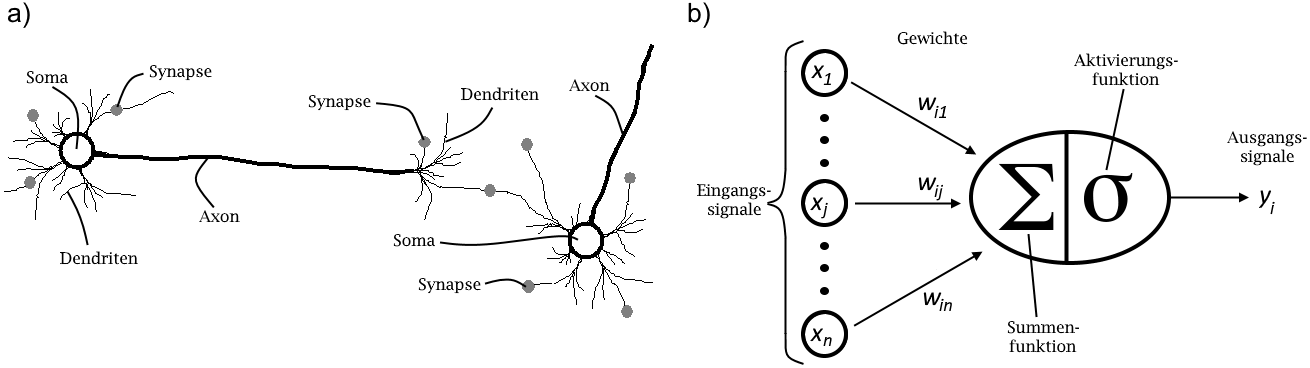
\includegraphics[width=0.5\textwidth]{Bilder/BNN_ANN.png}
    \caption{Gegenüberstellung eines Ausschnittes aus einem biologischen neuronalen Netz a)\protect\footnotemark{} und einem künstlichen neuronalen Netz b).}
    \label{fig:BNN_ANN}
\end{wrapfigure}

\addtocounter{footnote}{-1}%  -1 mal die Gesamtanzahl an Fußnoten in der wrapfigure
\addtocounter{Hfootnote}{-1}% -1 times total number of footnote(mark)s in the wrapfigure
\wrapfigfoot\footnotetext{\autoref{fig:BNN_ANN} a) und \autoref{tab:BNN_ANN} wurden aus\citet[2]{sen_an} übersetzt und angepasst.}
%\citet[\pno~2~ff.]{sen_an}

Es gibt Problemstellungen die mit klassischen mathematischen Modellen und Algorithmen gar nicht oder nur schwer zu lösen sind. Einige Beispiele wären die Gesichtserkennung oder die Erkennung von menschlicher Sprache. Unser Gehirn erkennt Gesichter und Sprachen aber anscheinend ohne größere Anstrengung.

\begin{wraptable}{l}{6.4cm}
    \caption {Analogie zwischen biologischen und künstlichen Neuronen.}
    \begin{tabular}{>{\centering\arraybackslash}m{2.2cm}>{\centering\arraybackslash}m{3.4cm}}
    \hline
    Biologisches\newline Neuron & Künstliches\newline Neuron            \\ \hline \hline
    Soma                & Summen- und\newline Aktivierungsfunktion      \\ 
    Dendrit             & Eingang                                       \\ 
    Axon                & Ausgang                                       \\ 
    Synapse             & Gewicht                                       \\ \hline
    \end{tabular}
    \label{tab:BNN_ANN}
\end{wraptable}

Aus der Untersuchung von biologischen Abläufen im Nervensystem von Wirbeltieren, wo Sinneseindrücke des Körpers aufgenommen und mit Hilfe diverser neuronaler Netze verarbeitet werden, entstanden Anfang der 40er Jahre des letzten Jahrhunderts künstliche neuronale Netze\fcite[A1.1:1]{Fiesler96} (engl. artificial neural networks)~(NN). 
\autoref{fig:BNN_ANN} zeigt eine Gegenüberstellung von künstlicher und biologischer neuronaler Netze und \autoref{tab:BNN_ANN} die Analogie der Bestandteile eines Neurons.

Künstliche neuronale Netze sind augenblicklich eine Disziplin der Computional Intelligence~(CI). Diese fasst verschiedene an die Natur angepasste Berechnungsmethoden zusammen. Weitere Methoden der CI sind Fuzzy-Systeme~(FS), Evolutionäre Algorithmen~(EA), Schwarmintelligenz~(SI) und Künstliche Immunsysteme~(AIS).\fcite[11 ff]{Kroll16} Obwohl sich diese Arbeit wesentlich mit NN beschäftigt, wird an dieser Stelle auf weitere CI-Methoden hingewiesen, da in der Literatur hybride CI-Systeme bekannt sind und auch genutzt werden.\\
%\lipsum

%\begin{figure}[h]
%	\centering
%	    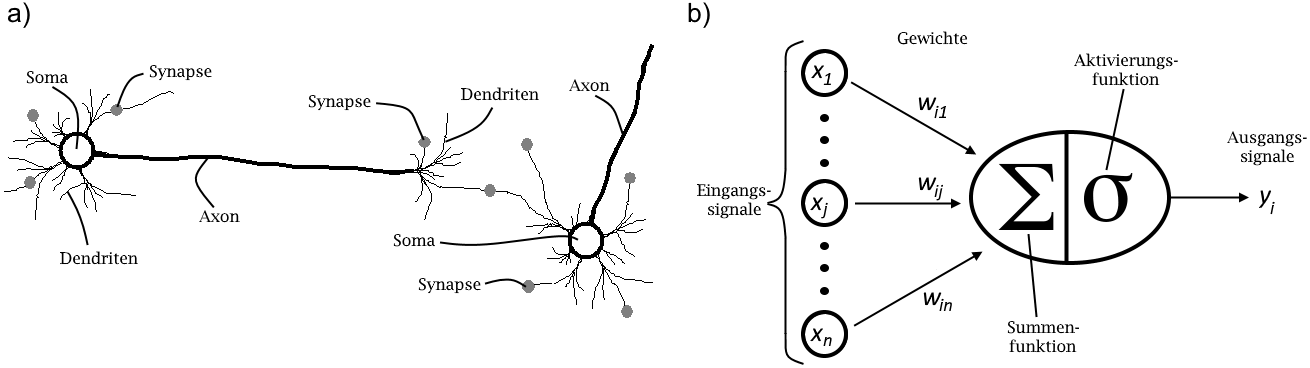
\includegraphics[width=0.5\linewidth]{Bilder/BNN_ANN.png}
%	\caption{Gegenüberstellung eines Ausschnittes aus einem biologischen neuronalen Netz a) und einem künstlichen neuronalen Netz b).}
%	\label{fig:BNN_ANN}
%\end{figure}



\subsection{Multilayerperzeptrons (MLP)}

\subsection{Radiale Basisfunktionen (RBF)}

\subsection{Gegenüberstellung von MLP- und RBF-Netzen}